\section{Data Acquisition and Conditioning} \label{sec:3}
\subsection{Open Data Retrieval}

The strain data used in this work were obtained from the LIGO Open Science Center (LOSC), which provides publicly available calibrated strain time series from the Advanced LIGO detectors. The data correspond to the event GW150914 at GPS time 1126259462.4.

For the primary analysis, a time window of $\pm 4$ seconds around the merger time was retrieved for both the Hanford (H1) and Livingston (L1) detectors. The strain time series is sampled at 4096 Hz in the public dataset, which is sufficient to resolve the frequency band of interest (30–300 Hz).

The strain $h(t)$ represents the dimensionless differential arm length variation,
\[
h(t) = \frac{\Delta L(t)}{L},
\]
where $L=4\,\mathrm{km}$ is the interferometer arm length.

The use of publicly released calibrated strain ensures reproducibility and consistency with the official analyses.

 
\begin{figure}[h]
	\centering
	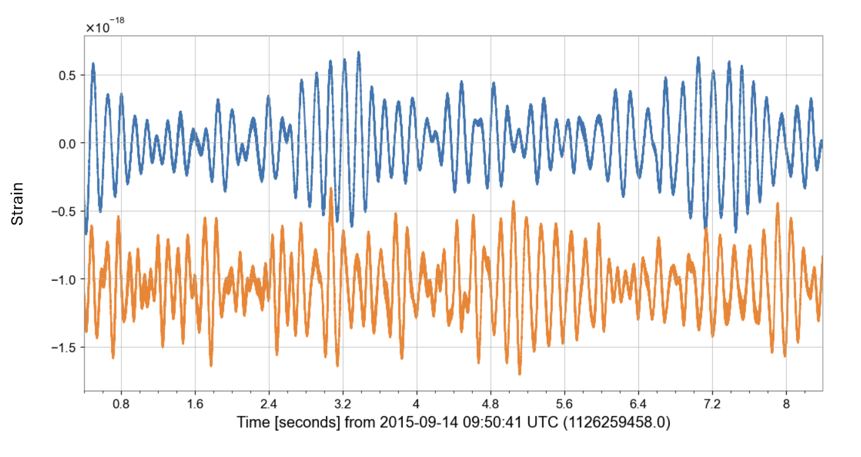
\includegraphics[width=0.85\textwidth]{figure/raw_strain.png}
	\caption{Raw strain data from H1 and L1 around GW150914 merger time (Blue: H1, Red: L1).}
\end{figure}


\subsection{Noise Characteristics and Power Spectral Density}

Gravitational-wave detectors operate in the presence of non-white, frequency-dependent noise. The statistical characterization of this noise is described by the one-sided power spectral density (PSD), $S_n(f)$, defined through
\[
\langle \tilde{n}(f)\tilde{n}^*(f') \rangle = \frac{1}{2} S_n(f)\delta(f-f'),
\]
where $\tilde{n}(f)$ is the Fourier transform of the detector noise.

The PSD is essential for optimal filtering because it quantifies the variance of noise as a function of frequency. In Advanced LIGO, the noise budget is dominated by seismic noise below $\sim 20$ Hz, thermal noise in the intermediate band, and quantum shot noise above several hundred Hz \cite{Aasi2015AdvancedLIGO}.

In this analysis, the PSD was estimated directly from the strain data  over a 8-second segment. The resulting PSD was interpolated to match the frequency resolution of the template waveforms and truncated at low frequencies to suppress spectral leakage. 

\begin{figure}[h]
	\centering
	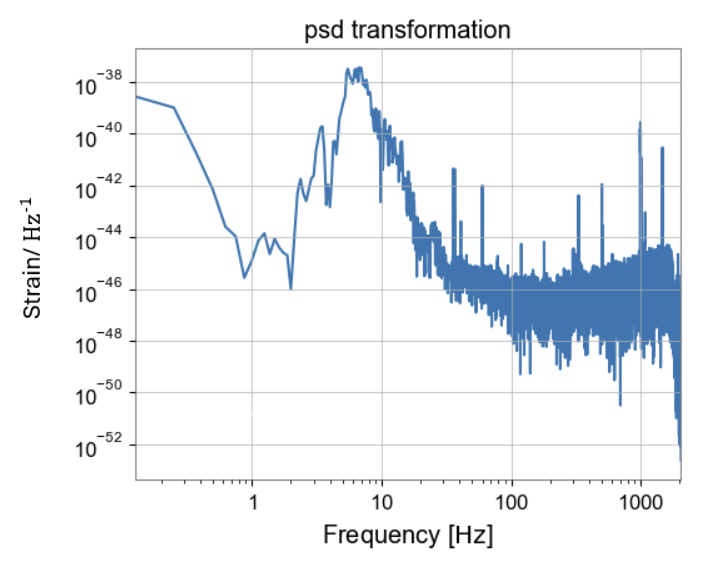
\includegraphics[width=0.8\textwidth]{figure/plot_psd.png}
	\caption{Estimated power spectral density of the H1 strain data.}
	\label{psd transformation}
\end{figure}


\subsection{Whitening Procedure}

Because detector noise is strongly frequency-dependent, direct time-domain analysis is essential. To equalize the noise variance across frequencies, the strain data were whitened by dividing the Fourier-domain data by the square root of the PSD:

\[
\tilde{h}_{\mathrm{white}}(f) = \frac{\tilde{h}(f)}{\sqrt{S_n(f)}}.
\]

This operation transforms colored noise into approximately unit-variance white noise. Whitening is essential for:

\begin{itemize}
	\item Visual identification of transient signals,
	\item Cross-correlation analysis between detectors,
	\item Time–frequency representations such as the Q-transform.
\end{itemize}

After whitening, the noise background becomes approximately stationary with uniform variance across frequencies.

\subsection{Bandpass and Notch Filtering}

Although whitening suppresses frequency-dependent noise, residual contributions outside the astrophysically relevant band remain. For binary black hole mergers similar to GW150914, most detectable signal power lies between approximately 30 Hz and 300 Hz. From fig \ref{psd transformation}, the best frequency window to study is something between 50 to 300 Hz\cite{Abbott2016Discovery,Abbott2016Properties}. 

Therefore, a bandpass filter between 50 Hz and 300 Hz was applied to the strain data. The lower cutoff reduces contamination from seismic and suspension noise, while the upper cutoff removes high-frequency shot noise.

In addition, a narrow notch filter at 60 Hz was applied to suppress contamination from power-line harmonics, which are a known environmental noise source in ground-based interferometers \cite{Aasi2015AdvancedLIGO}.

After bandpass and notch filtering, the waveform morphology of GW150914 becomes clearly visible in the time domain over a $\sim 2$ s interval surrounding the merger.


\begin{figure}[h]
	\centering
	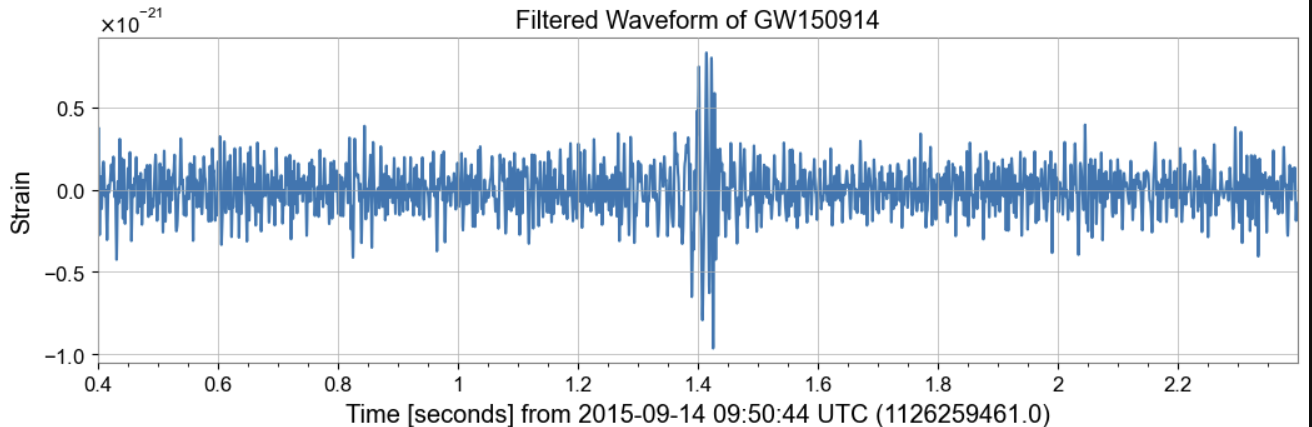
\includegraphics[width=0.85\textwidth]{figure/filtered_waveform}
	\caption{Bandpass and notch filtered strain signal near GW150914.}
	\label{filtered data}
\end{figure}


\subsection{Data Preparation for Subsequent Analysis}

Following conditioning, the strain data were cropped to shorter windows around the merger time for specific analyses:

\begin{itemize}
	\item $\pm 1$ ms window for cross-correlation time-delay measurement,
	\item $\pm 1$ s window for Q-transform analysis,
	\item $\pm 32$ s window for matched filtering and chi-square estimation.
\end{itemize}

Each time window was selected based on the statistical requirements of the corresponding method. Short windows minimize contamination from unrelated noise transients, while longer segments are necessary for stable PSD estimation and matched filtering.

This conditioned dataset forms the basis for the time-delay analysis presented in the next section.
